\chapter{Desenvolvimento do tema}
\label{cap:experiments}

Este capítulo é opcional e, a existir, é aqui que deve descrever como é que o seu projecto evoluiu.

O projeto é constituido em quatro partes:

\begin{itemize}
    \item \textit{"Port Controller"} - daemon em C\#;
    \item API e Interface Web;
    \item Sitema de notificações;
    \item Ambiente de teste do projeto;
\end{itemize}

\section{Port Controller}

\subsection{Escolha da tecnologia}

Uma vez que a plataforma forge funciona no sistema \textit{Alpine Linux} seria
necessário escolher ferramentas suportadas por esta distribuição.

No caso deste componente do projeto foi escolhida a linguagem C\# com o 
\textit{framework} .NET Core versão 7.0.


\subsection{Funcionalidades}

O \textit{"Port Controller"} tem como principal função estar à escuta de pedidos do
administrador e executar estes pedidos no \textit{container} selecionado. Os 
pedidos são recebidos na componente da \textit{unix socket} em formato
\textit{JSON}.

O \textit{Port Controller} é também capaz de interagir com \textit{containers}
do tipo LXD, e Incus e executar comandos dentro destes para interagir com a
\textit{FireWall} Iptables ou Nftables.

\subsection{Estrutura do código}

O código do "Port Controller" é constituido pelos seguintes ficheiros:

\begin{itemize}
    \item Program.cs;
    \item SocketData.cs;
    \item Containers.cs;
    \item Lxc.cs;
    \item Incus.cs;
\end{itemize}

\subsection{Funcionamento do código}


No Ficheiro Program na função \textit{main} está defenido o caminho do ficheiro 
da unix socket que permite a comunição entre o \textit{"Port Controller"} e 
a interface \textit{Web} ou API.

\begin{figure}
\begin{center}
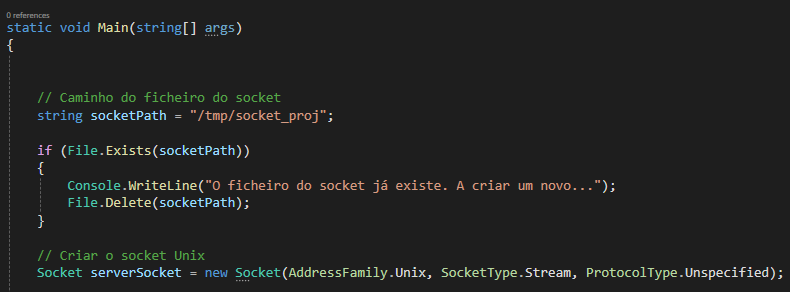
\includegraphics[width=13cm]{figs/codigo_pc.png}
\caption{Codigo Port Controller}
\end{center}
\end{figure}




As classes Lxc e Incus recebem herença da classe Containers.


\section{API e Interface Web}

\subsection{Estrutura da API}

\subsection{Formato do JSON}


\section*{Sumário}

Ver o \nameref{sec:intro_summary} página \pageref{sec:intro_summary} para perceber como utilizar esta secção.


